\chapter{UML Class diagram}
How to identify important concepts on the environment:
\begin{enumerate}
\item Underline nouns: nouns are candidates for classes, attributes, \dots;
\item Define classes;
\item Define attributes for classes;
\item Underline verbs: verbs are candidates for relationships;
\item Define relationships;
\item Define multiplicities.
\end{enumerate}

\section{University}
Define a class diagram for a glossary for university. In a university there are different classrooms, offices and departments. A department has a name and it contains many offices. A person working at the university has a unique ID and can be a professor or an employee.

\begin{itemize}
\item A professor can be a full, associate or assistant professor and he/she is enrolled in one department.
\item Offices and classrooms have a number ID
\item A classroom has a number of seats.
\item Every Employee works in an office.
\item An employee enters and exits a classroom.
\end{itemize}

\subsection{Solution}
Define a class diagram for a glossary for \colorbox{yellow}{university}. In a university there are different \colorbox{yellow}{classrooms}, \colorbox{yellow}{offices} and \colorbox{yellow}{departments}. A department has a \colorbox{cyan}{name} and it \colorbox{green}{contains} many offices. A \colorbox{yellow}{person} \colorbox{green}{working} at the university has a unique \colorbox{cyan}{ID} and can be a \colorbox{yellow}{professor} or an \colorbox{yellow}{employee}.

\begin{itemize}
\item A professor can be a full, associate or assistant professor and he/she \colorbox{green}{is enrolled} in one department.
\item Offices and classrooms have a number \colorbox{cyan}{ID};
\item A classroom has a \colorbox{cyan}{number of seats}.
\item Every employee \colorbox{green}{works} in an office.
\item An employee \colorbox{green}{enters and exits} a classroom.
\end{itemize}

A possible strategy to represent different professor roles is to have a type field in the \emph{Professor} class or use a generalization-specialization pattern to identify the possible types. If there is no peculiar properties in the sub-classes, it is good practice to avoid the use of specialization. A ``discriminant'' attribute should be sufficient and it is preferable.

\begin{figure}[hbtp]
\centering
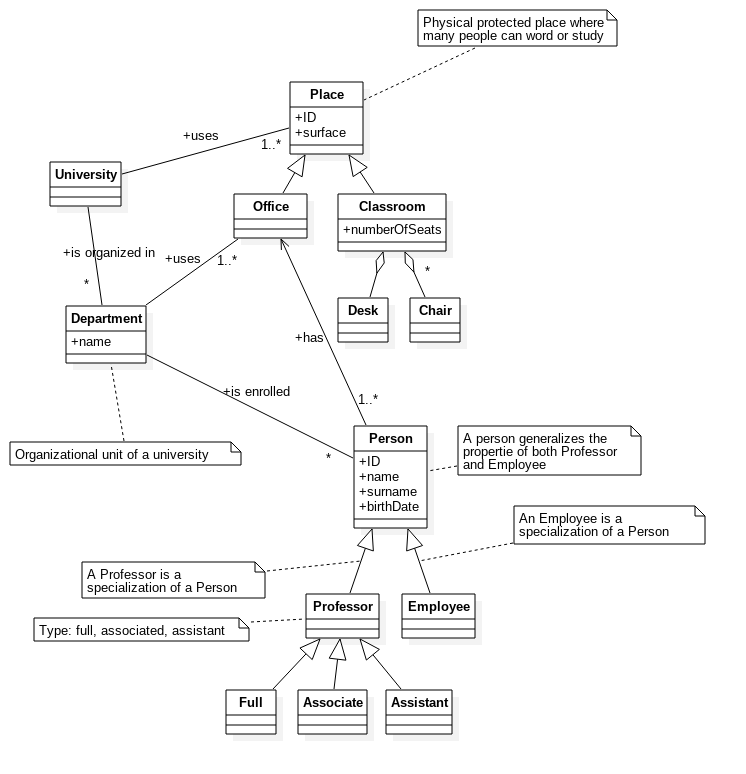
\includegraphics[scale=0.45]{exercises/classDiagram_university.png}
\caption{University - Class Diagram}
\end{figure}

\newpage
\section{Flights}
Draw a class diagram to define the glossary for management of flights and pilots.

An airline operates flights. Each airline has an ID. Each flight has an ID, a departure airport and an arrival airport: an airport has a unique identifier. Each flight has a pilot and a co-pilot, and it uses an aircraft of a certain type; a flight has also a departure time and an arrival time.

An airline owns a set of aircrafts of different types. An aircraft can be in a working state or it can be under repair, and in a particular moment an aircraft can be landed or airborne.

A company has a set of pilots: each pilot has an experience level: 1 is minimum, 3 is maximum.

A type of aircraft may need a particular number of pilots, with a different role (Ex. captain, co-pilot, navigator): there must be at least one captain and one co-pilot, and a captain must have a level 3.

\begin{sidewaysfigure}
\centering
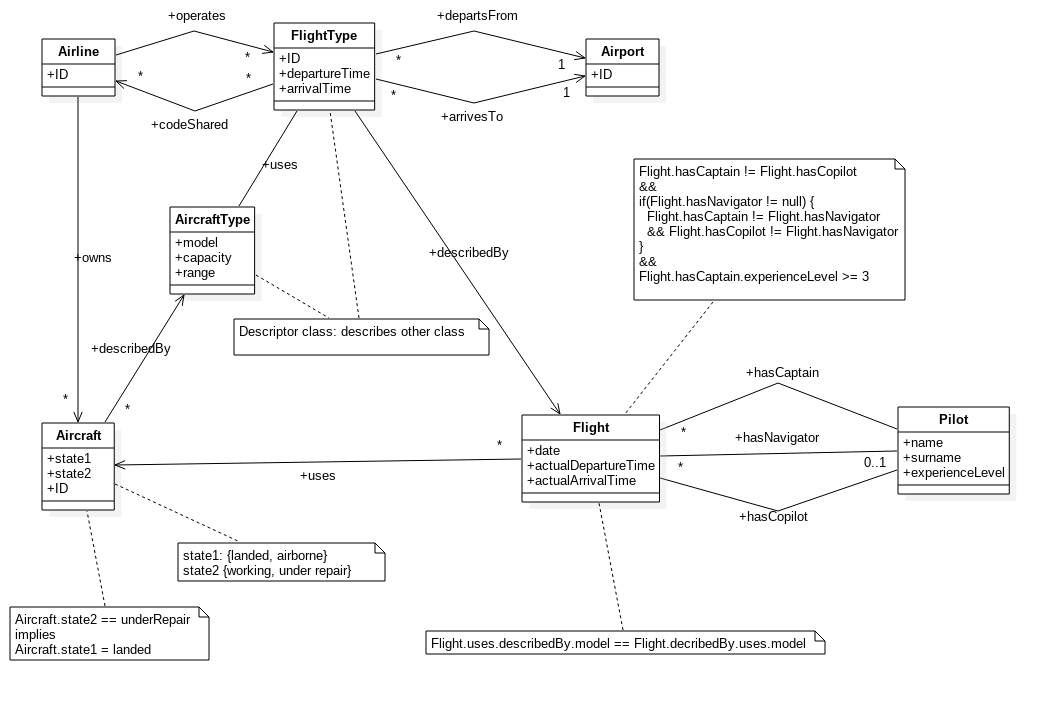
\includegraphics[scale=0.5]{exercises/classDiagram_flights.png}
\caption{Flights - Class Diagram}
\end{sidewaysfigure}